\newpage
\section{Scaling Area}

\fixnote{Include here or in the notes some content of the PowerPoint.  Need a scaling volume activity.  See comments for a start.}

\begin{prob}
Is a $3\times 5$ rectangle similar to a $4\times 6$ rectangle?  Explain your reasoning.  Now come up with another explanation. 
\end{prob}

\vspace{.5in} 

\begin{prob}
Use area formulas to explain what happens to the area of a rectangle under scaling by a factor of $k$?  What about a triangle?  What about a circle?  
\end{prob}

\begin{prob}
Below is a figure and a dilation of that figure about point $O$.  
\[
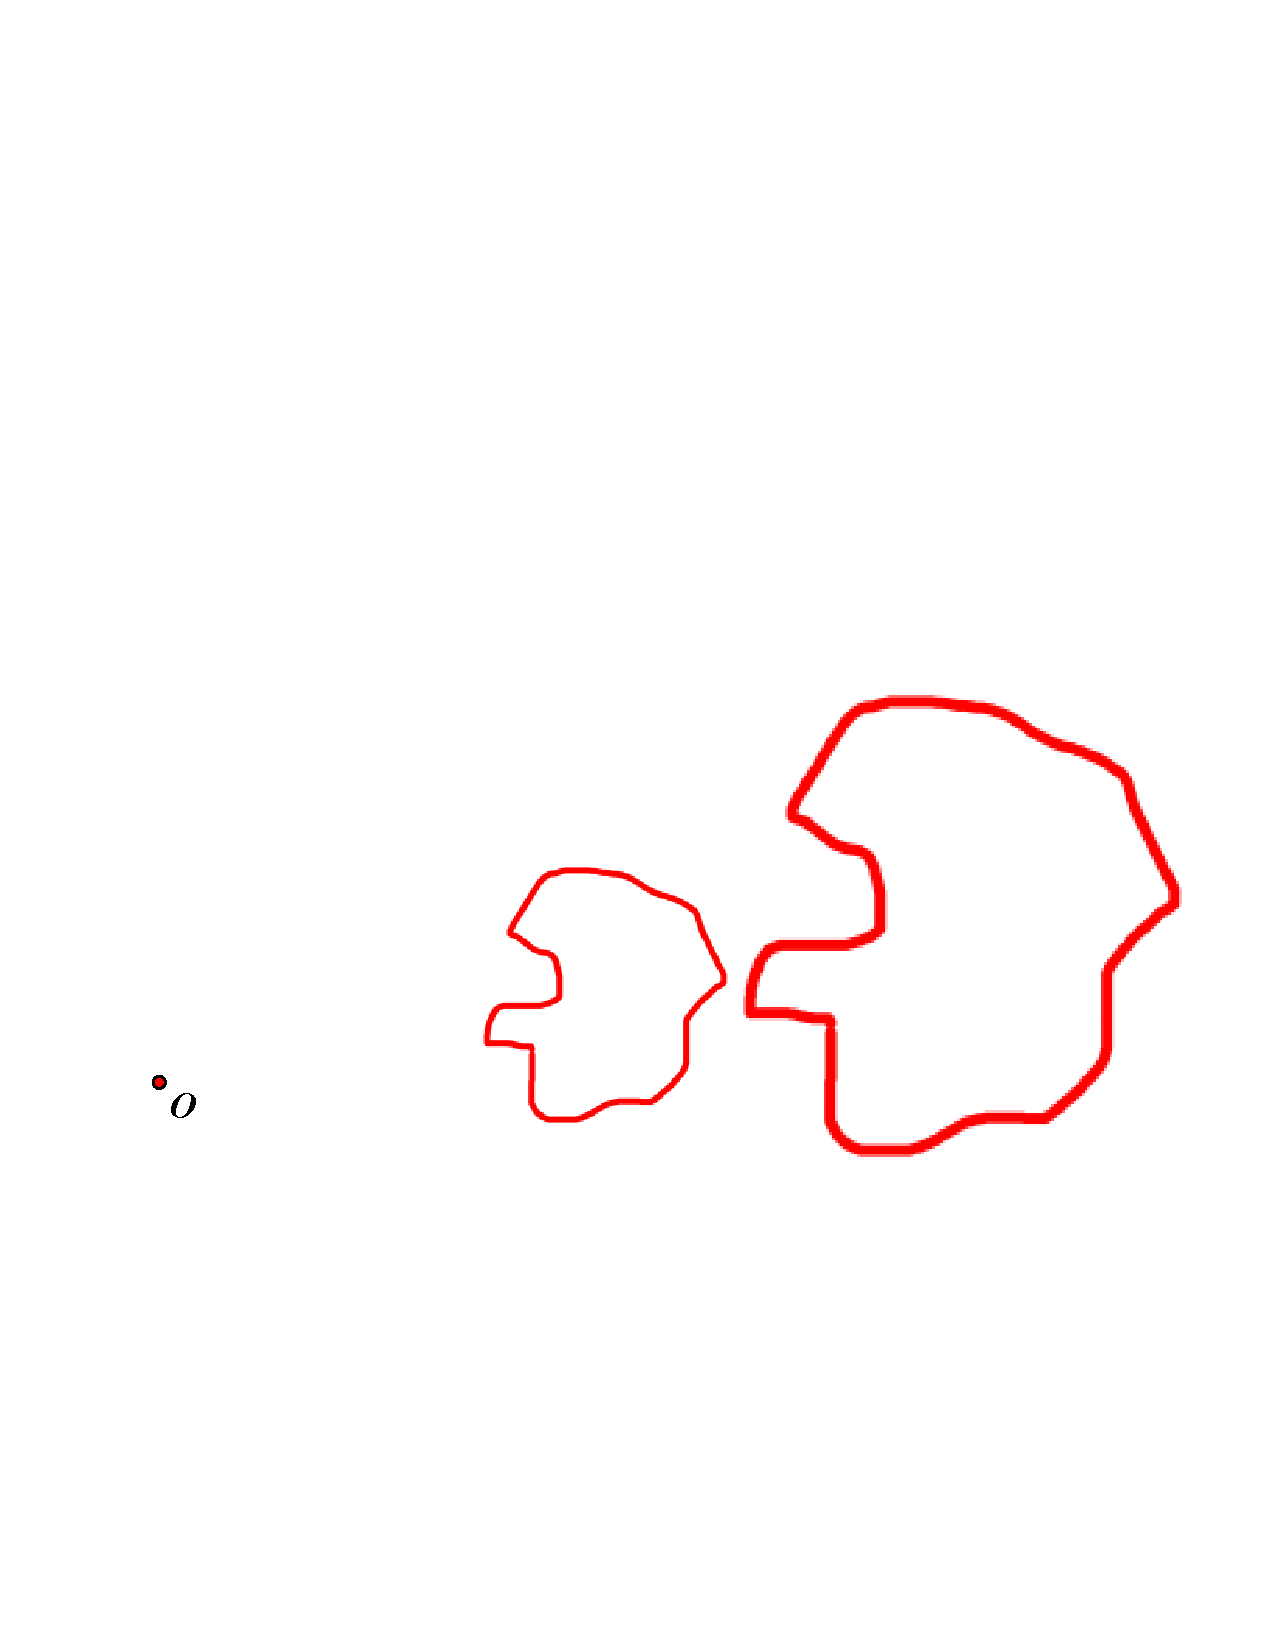
\includegraphics{../graphics/dilation.pdf}
\]
\begin{enumerate}
\item Find the scale factor of the dilation.  Explain your reasoning. 
\item What can you say about the areas of the two figures?  Explain your reasoning. 
\end{enumerate}
\end{prob}


%\begin{prob}
%Imagine a $2\times 3\times 4$ right rectangular prism.  
%\begin{enumerate}
%\item Find the volume of the prism.  From the meaning of volume, explain why your calculations make sense.  
%\item Explain generally why the volume formula makes sense for dimensions that are counting numbers.  
%\item If you scale the prism by a factor of 3, how many copies of the original prism can you fit in the new one?  What does that say about the volume of the new prism?   
%\end{enumerate}
%\end{prob}

